\documentclass[12pt]{article}
\usepackage[utf8]{inputenc}
\usepackage[T1]{fontenc}
\usepackage[a4paper, left=2.4cm, right=2.4cm, top=2cm, bottom=2cm, nomarginpar]{geometry}
\usepackage{amsmath, algorithm, pgfplots, pgf, pdfpages, amsfonts, amssymb, stmaryrd, enumitem,graphicx, algpseudocode, setspace, listings, courier, color, caption, centernot, hyperref, lstautogobble, zi4, mathtools, lmodern, colortbl, array, multicol, fancyhdr, lastpage, svg}
\usepackage{booktabs}
\hypersetup{
    pdftitle={CE204_FP1_G6},
    pdftoolbar=true,        % show Acrobat’s toolbar?
    pdfmenubar=true,        % show Acrobat’s menu?
    pdfauthor={Muhammet Yağcıoğlu},
    pdfsubject={CE204_FP_RPs},
    pdfcreator={Muhammet Yağcıoğlu},   % creator of the document
    pdfproducer={Muhammet Yağcıoğlu}, % producer of the document
    colorlinks,
    linkcolor={black},
    citecolor={black},
    urlcolor={blue!80!black}
}
\usepackage[noblocks]{authblk}
\usepackage[version=4]{mhchem}
\usepackage[export]{adjustbox}
\usepackage{eso-pic} % Required for absolute positioning
\graphicspath{ {./images/} }
\usetikzlibrary{patterns}
\usepackage{tikz-3dplot}
\usepackage[version=4]{mhchem}
\usepackage[export]{adjustbox}
\usepgfplotslibrary{groupplots}
\usepackage{xcolor}
\usepackage[absolute,overlay]{textpos}
\usepackage{ragged2e}
\usepackage{xcolor}
\usepackage{amsthm}
\usepackage{tikz}




%----------compiler settings---------
\setlength{\parindent}{0pt}
\everymath{\displaystyle}
\onehalfspacing

%-----------colors----------
\pgfplotsset{compat=1.18}
\definecolor{bluekeywords}{rgb}{0.13, 0.13, 1}
\definecolor{greencomments}{rgb}{0, 0.5, 0}
\definecolor{redstrings}{rgb}{0.9, 0, 0}
\definecolor{graynumbers}{rgb}{0.5, 0.5, 0.5}
\definecolor{bronze}{rgb}{0.82, 0.41, 0.12}
\definecolor{crimson}{rgb}{0.86, 0.08, 0.24}
\definecolor{brown(web)}{rgb}{0.65, 0.16, 0.16}
\definecolor{darkspringgreen}{rgb}{0.16, 0.32, 0.75}
\definecolor{blue(ncs)}{rgb}{0.0, 0.53, 0.74}
\definecolor{amber}{rgb}{1.0, 0.49, 0.0}
\definecolor{cadmiumgreen}{rgb}{0.0, 0.42, 0.24}




%-------code frame-----------
\lstset{
    autogobble,
    columns=fullflexible,
    showspaces=false,
    showtabs=false,
    breaklines=true,
    showstringspaces=false,
    breakatwhitespace=true,
    escapeinside={(*@}{@*)},
    commentstyle=\color{greencomments},
    keywordstyle=\color{bluekeywords},
    stringstyle=\color{redstrings},
    numberstyle=\color{graynumbers},
    basicstyle=\ttfamily\footnotesize,
    frame=l,
    framesep=12pt,
    xleftmargin=12pt,
    tabsize=4,
    captionpos=b
}



\lstdefinelanguage{myMMA}{
keywords={SetDirectory, NotebookDirectory, Exp, IdentityMatrix, Eigenvalues, 
ListPlot, PlotRange, PlotStyle, Directive, PointSize, AspectRatio, Blue, Graphics, Line, 
Manipulate, Show, Sqrt, UniformDistribution, GammaDistribution, BetaDistribution, 
Nintegrate, For, DataRange, AxesLabel, PlotLabel, Transpose, Export, Plot, Append, Infinity},
keywordstyle=\color{black},
commentstyle=\color{gray}, 
identifierstyle=\color{blue},
sensitive=false,
comment=[l]{(*},
morecomment=[s]{/*}{*/},
morestring=[b]',
morestring=[b]"
}






%-----gauss declare---------
\pgfmathdeclarefunction{gauss}{2}{%
  \pgfmathparse{1/(#2*sqrt(2*pi)) * exp(-((x-#1)^2)/(2*#2^2))}%
}
\usetikzlibrary{arrows.meta, decorations.markings}
\pgfplotsset{compat=1.17}







%--------------page numbering------------
\fancyfoot[R]{page \thepage\ of \textcolor{bronze}{\pageref{LastPage}}}
\fancyhead[R]{Group 6}



%-------------qframe settings---------------

\usepackage[framemethod=TikZ]{mdframed}
\newmdenv[%
    skipabove=1em, % space above the frame
    skipbelow=1em, % space below the frame
    linewidth=1pt, % width of the frame lines
    linecolor=gray!80, % color of the frame lines
    backgroundcolor=gray!9, % background color inside the frame
    roundcorner=5pt, % radius of the rounded corners
    innerleftmargin=1em, % margin within the frame at the left
    innerrightmargin=1em, % margin within the frame at the right
    innertopmargin=0.5em, % margin within the frame at the top
    innerbottommargin=0.5em % margin within the frame at the bottom
]{qframe}

\newenvironment{q}
{
    \begin{qframe}
    \noindent\textit{\textbf{Problem Statement:}}
    \par\smallskip
}
{
    \end{qframe}
}





%-------------ANSWER TAG---------------
\newcommand{\AnswerTag}{\hfill 
\begin{tikzpicture} \fill[black] (0.35cm,0) -- (0,0.175cm) -- (0.35cm,0.35cm) -- cycle;\end{tikzpicture}}



%-------Theorem and another question frames----------
\newenvironment{theorem}{\begin{mdframed}\textbf{Theorem.}}{\end{mdframed}}

%usage: \begin{theorem}

\newenvironment{question}{\begin{mdframed}\textbf{Question.}}{\end{mdframed}}

%usage: %usage: \begin{question}
\usepackage{hyperref} 
 \hypersetup{ 
     colorlinks=true, 
     linkcolor=blue, 
     filecolor=blue, 
     citecolor = black,       
     urlcolor=cyan, 
     } 
\usepackage{sectsty}
\title{\vspace{-1cm}CE231 - Engineering Economy HW1}
\author{Muhammet Yağcıoğlu - 290204042}

\fancyhead[L]{\textbf{CE 231, Engineering Economy, Fall 2023, HW1}}


\begin{document}
\pagestyle{fancy}
\maketitle\thispagestyle{fancy}

\tableofcontents

\newpage
\subsection*{Question 1}
\addcontentsline{toc}{section}{Question 1}
\begin{q}
How long does it take for an initial investment of \(\$ 5,000\) to quadruple,

(a) when the interest rate is \(8 \%\) per year?

(b) when the interest rate is \(10 \%\) per year, compounded monthly?

(c) when the interest rate is \(12 \%\) per year, compounded continuously?
\end{q}


\begin{figure}[!ht]
    \centering
    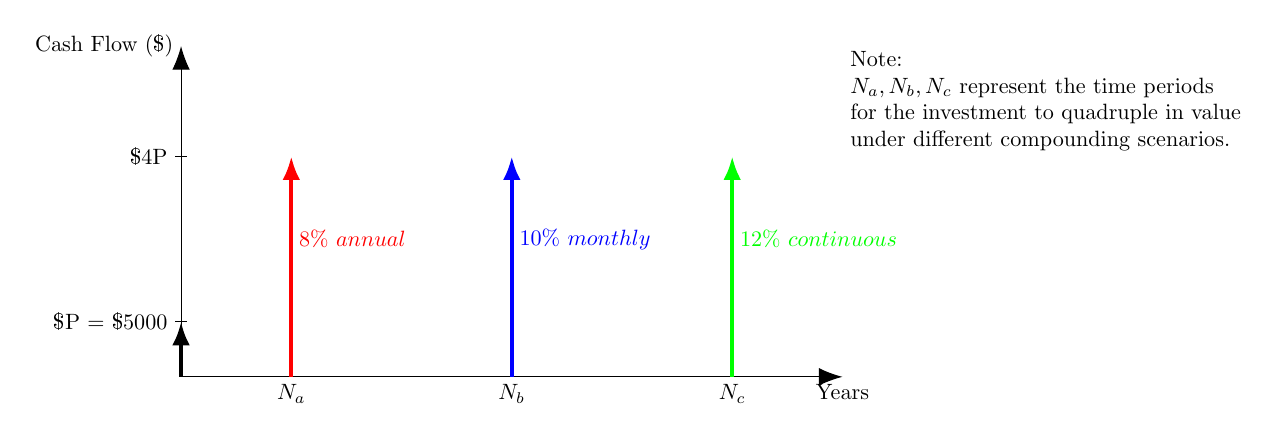
\begin{tikzpicture}[scale=0.7, every node/.style={scale=0.8}]
        % Draw axes
        \draw[-{Latex[length=3mm]}] (0,0) -- (12,0) node[anchor=north] {Years};
        \draw[-{Latex[length=3mm]}] (0,0) -- (0,6) node[anchor=east] {Cash Flow (\$)};

        % Mark initial investment (P) and quadruple value (4P)
        \draw (3pt,1) -- (-3pt,1) node[anchor=east] {\$P = \$5000};
        \draw (3pt,4) -- (-3pt,4) node[anchor=east] {\$4P};

        % Initial investment arrow
        \draw[black, line width=0.5mm, -{Latex[length=3mm]}] (0,0) -- (0,1);

        % Time periods
        \node[anchor=north] at (2,0) {\(N_a\)};
        \node[anchor=north] at (6,0) {\(N_b\)};
        \node[anchor=north] at (10,0) {\(N_c\)};

        % Cash flow arrows for 8% annual
        \draw[red, line width=0.5mm, -{Latex[length=3mm]}] (2,0) -- (2,4);
        \node[red, anchor=west] at (2, 2.5) {\(8\%\ annual\)};

        % Cash flow arrows for 10% monthly
        \draw[blue, line width=0.5mm, -{Latex[length=3mm]}] (6,0) -- (6,4);
        \node[blue, anchor=west] at (6, 2.5) {\(10\%\ monthly\)};

        % Cash flow arrows for 12% continuous
        \draw[green, line width=0.5mm, -{Latex[length=3mm]}] (10,0) -- (10,4);
        \node[green, anchor=west] at (10, 2.5) {\(12\%\ continuous\)};

        % Annotations for continuous and monthly compounding
        \node[align=left, anchor=west] at (12,5) {
            Note: \\
            \( N_a, N_b, N_c \) represent the time periods \\
            for the investment to quadruple in value \\
            under different compounding scenarios.};

    \end{tikzpicture}
    \caption{}
    \label{fig:enhanced-investment-growth}
\end{figure}


Let \( P_0 \) be the initial principal amount of \$5,000 and let \( P \) be the final amount, which in the case of quadrupling is \$20,000. The relationship between \( P_0 \), \( P \), the interest rate \( r \), and the time period \( N \) in years for an investment compounding annually is given by,

\[
P = P_0(1 + r)^N.
\]

For an investment compounding \( M \) times per year, the relationship becomes

\[
P = P_0\left(1 + \frac{r}{M}\right)^{MN}.
\]

In the case of continuous compounding, the relationship is described by

\[
P = P_0 e^{rN}.
\]

(a) For an annual interest rate of 8\% (\( r = 0.08 \)) with annual compounding, we set \( P = 4P_0 \) and solve for \( N \)

\[
\therefore 4P_0 = P_0(1 + 0.08)^{N_a} \implies 4 = (1.08)^{N_a} \implies N_a = \frac{\ln 4}{\ln 1.08} \approx 18.0129.
\]

(b) For a monthly compounded interest rate of 10\% (\( r = 0.10 \)), with \( M = 12 \) (months per year), we solve for \( N \)

\[
\therefore 4P_0 = P_0\left(1 + \frac{0.10}{12}\right)^{12N_b} \implies 4 = \left(1 + \frac{0.10}{12}\right)^{12N_b} \implies N_b = \frac{\ln 4}{12 \ln \left(1 + \frac{0.10}{12}\right)} \approx 13.9206.
\]

(c) For a continuously compounded interest rate of 12\% (\( r = 0.12 \)),

\[
\therefore 4P_0 = P_0 e^{0.12N_c} \implies 4 = e^{0.12N_c} \implies N_c = \frac{\ln 4}{0.12} \approx 11.5525.
\]

\newpage
\subsection*{Question 2}
\addcontentsline{toc}{section}{Question 2}
\begin{q}
A couple with a newborn daughter wants to establish a college fund to pay for future college expenses. The couple can earn \(12 \%\) compounding annually on their investments and estimate that future college costs will be \(\$ 50,000\) per year for four years. Assume that the daughter enters college at age 18 and that payments are made on each birthday. Also, assume that college costs must be paid at the beginning of the college year. What annual payment must be made to ensure that a sufficient amount has been saved to cover all costs when the daughter enters college? [Make sure to begin by drawing the correct cash-flow diagram.]
\end{q}


\begin{figure}[!ht]
    \centering
    \begin{tikzpicture}[scale=1.3, every node/.style={scale=1}]
        % Draw axes
        \draw[-{Latex[length=3mm]}] (0,0) -- (10,0) node[anchor=north] {Years};
        \draw[-{Latex[length=3mm]}] (0,-3) -- (0,3) node[anchor=east] {Cash Flow (\$)};
    
        % Draw initial interval (0,5)
        \foreach \x in {0,1,...,5} {
            \draw (\x,3pt) -- (\x,-3pt);
            \node[anchor=east] at (\x,0) {\x};
        }
    
        % Payments (P) in initial years from 1 to 18
        \foreach \x in {1,...,4} {
            \draw[red, line width=0.5mm, -{Latex[length=3mm]}] (\x,0) -- (\x,-1.75);
            \node[red] at (\x, -2) {\scriptsize \$P};
        }
        \foreach \x in {6} {
            \draw[red, line width=0.5mm, -{Latex[length=3mm]}] (\x,0) -- (\x,-1.75);
            \node[red] at (\x, -2) {\scriptsize \$P};
        }
    
        % Jagged line to indicate continuation
        \draw[decorate, decoration={zigzag,segment length=4,amplitude=.9}, -{Latex[length=3mm]}] 
        (5,0) -- (6,0);
    
        % Draw final interval (17,21)
        \foreach \x in {18,19,20,21} {
            \draw (\x - 12,3pt) -- (\x - 12,-3pt);
            \node[anchor=east] at (\x - 12,0) {\x};
        }
    
        % Payment (P) in last year before college
        \draw[red, line width=0.5mm, -{Latex[length=3mm]}] (5,0) -- (5,-1.75);
        \node[red] at (5, -2) {\scriptsize \$P};
    
        % College costs (D) from year 18 to 21
        \foreach \x in {18,19,20,21} {
            \draw[blue, line width=0.5mm, -{Latex[length=3mm]}] (\x - 12,0) -- (\x - 12,1.65);
            \node[blue] at (\x - 12, 2) {\scriptsize \$D};
        }
    
        % Add labels
        \node[anchor=east] at (0, -0.75) {\scriptsize Annual Payments};
        \node[anchor=east] at (0, 0.75) {\scriptsize College Costs};
    
    \end{tikzpicture}
    \caption{Cash flow diagram for a college fund. Annual payments are made for the first 18 years, followed by college costs in years 18 to 21.}
    \label{fig:college-fund-cash-flow}
\end{figure}






Let \( D \) be the annual deposit amount required, \( r \) the annual interest rate, \( n \) the number of years until the child enters college, and \( m \) the duration of college requiring annual payments. In this, \( r = 12\% = 0.12 \), \( n = 18 \), \( m = 4 \), and the annual college cost is \( \$50,000 \). To find \( D \), consider the present value of the deposits and the withdrawals. This can be seen as the equivalent as two distinct diagrams for college expenses and investment cash flow.  The present value \( P \) of a series of equal annual payments made at the end of each year for \( n \) years, compounded annually at an interest rate \( r \), is given by:

\[ Q = P \cdot \frac{1 - (1 + r)^{-n}}{r} \]

The present value \( W \) of the withdrawals required for college, which start at the beginning of the 18th year, is calculated similarly, but with the same formula we find the present value of withdrawals in the \(n-1\)st year. To apply this to year \(0\), multiply it by the \(n-1\)st order of the simple present-future coefficient. Thus, \( D \) is the product of the present value of the college costs over \(4\) years, discounted back \(17\) years (since the first withdrawal is at the beginning of the 18th year):

\[ W = D \cdot \frac{1 - (1 + r)^{-m}}{r} \cdot (1 + r)^{-(n-1)} \]

Equating the present values of the deposits and withdrawals yields:
\[Q=W\]
\[ P \cdot \frac{1 - (1 + r)^{-n}}{r} = 50,000 \cdot \frac{1 - (1 + r)^{-m}}{r} \cdot (1 + r)^{-n+1} \]

Solving for \(P\) and substituting \( r = 0.12 \), \( n = 18 \), and \( m = 4 \):


\[\therefore P = \frac{50000(1+r)^{1-m}\left(-1+(1+r)^m\right)}{-1+(1+r)^n} = \boxed{3050.9854}.\]

























\newpage
\subsection*{Question 3}
\addcontentsline{toc}{section}{Question 3}
\begin{q}
A firm has available the following set of investment options. Additionally, the firm can always lend money to other firms, thereby receiving a return of \(6 \%\). Or they can borrow up to \(\$ 100,000\) at a rate of \(10 \%\). What should the firm's MARR be if they had a budget for projects of \(\$ 40,000\) ?

\begin{center}
\begin{tabular}{ccc} 
Project & Invesment & Rate of Return \\
1 & \(\$ 10,000\) & \(20 \%\) \\
2 & \(\$ 10,000\) & \(15 \%\) \\
3 & \(\$ 10,000\) & \(10 \%\) \\
4 & \(\$ 10,000\) & \(8 \%\) \\
5 & \(\$ 10,000\) & \(7 \%\) \\
6 & \(\$ 10,000\) & \(4 \%\)
\end{tabular}
\end{center}
\end{q}


\begin{figure}[!ht]
    \centering
    \begin{tikzpicture}[scale=0.9, every node/.style={scale=0.4}]
        % Draw axes
        \draw[-{Latex[length=3mm]}] (0,0) -- (12,0) node[anchor=north] {Projects};
        \draw[-{Latex[length=3mm]}] (0,-5) -- (0,5) node[anchor=east] {Cash Flow (\$)};

        % Initial budget
        \draw[black, line width=0.5mm, -{Latex[length=3mm]}] (0,0) -- (0,3);
        \node[black, anchor=east] at (0, 1.5) {Budget \$40,000};

        % Investment options
        \foreach \x/\y/\rate in {1/1/20\%, 2/2/15\%, 3/3/10\%, 4/4/8\%, 5/5/7\%, 6/6/4\%} {
            \draw[blue, line width=0.5mm, -{Latex[length=3mm]}] (\x,0) -- (\x, -2);
            \node[blue, anchor=east] at (\x, -1) {\$10,000, \rate};
        }

        % Lending option
        \draw[green, line width=0.5mm, -{Latex[length=3mm]}] (10,0) -- (10,2);
        \node[green, anchor=west] at (10, 1) {Lend at 6\%};

        % Borrowing option
        \draw[red, line width=0.5mm, -{Latex[length=3mm]}] (11,0) -- (11,-3);
        \node[red, anchor=west] at (11, -1.5) {\$100,000 at 10\%};

        % MARR Consideration
        \node[align=left, anchor=west] at (12,5) {
            Note: \\
            Investment choices should be based on \\
            the firm's Minimum Acceptable Rate of Return (MARR).};

    \end{tikzpicture}
    \caption{Cash flow diagram representing a firm's investment options, lending and borrowing possibilities.}
    \label{fig:firm-investment-options}
\end{figure}


Let the firm have a set of investment options \( \{P_1, P_2, P_3, P_4, P_5, P_6\} \), with each project \( P_i \) requiring an investment \( I_i \) and offering a rate of return \( R_i \). Additionally, the firm can lend money at a rate of \( r_L = 6\% \) or borrow up to \( \$100,000 \) at a rate of \( r_B = 10\% \). The firm's budget for projects is \( B = \$40,000 \). Given:
\begin{align*}
I &= \{10000, 10000, 10000, 10000, 10000, 10000\} \text{ (in \$)}, \\
R &= \{20\%, 15\%, 10\%, 8\%, 7\%, 4\%\}.
\end{align*}

The firm should select projects that maximize its return, given the constraint of its budget. This problem is a linear programming problem. Consider a firm with an array of investment opportunities, \( \mathcal{P} = \{ P_1, P_2, \ldots, P_n \} \), where each project \( P_i \) demands an investment \( I_i \) and proffers a rate of return \( R_i \). The firm's budgetary constraint is represented by \( B \), and it has the additional options of lending at a rate \( r_L \) and borrowing at a rate \( r_B \), up to a ceiling \( L \). Introduce binary decision variables \( x_i \) for each project \( P_i \), where \( x_i = 1 \) signifies the selection of the project, and \( x_i = 0 \) its non-selection. The aim is to maximize the total return,

\[
\text{Maximize} \quad Z = \sum_{i=1}^{n} R_i I_i x_i \quad \text{subject to} \quad \sum_{i=1}^{n} I_i x_i \leq B \quad \text{and} \quad x_i \in \{0, 1\} \, \forall i.
\]

When we solved this optimization quandary, the sum investment \( T \) is computed as \( T = \sum_{i=1}^{n} I_i x_i^* \), where \( x_i^* \) denotes the optimal choice for each project. The MARR is hence defined,

\[
\text{MARR} = 
\begin{cases} 
\min \{ R_i \mid x_i^* > 0 \}, & \text{if } T = B \\
\max(\min \{ R_i \mid x_i^* > 0 \}, r_L), & \text{if } T < B.
\end{cases}
\]

Applying the optimization model to this set of projects with the given budget constraint \( B = \$40,000 \), we select the projects offering the highest returns within the budget.

\begin{center}
\begin{algorithm}
\caption{Determine \(MARR\)}
\begin{algorithmic}[1]
\Require $P, I, R, B, r_L, r_B, L$
\State Sort $P$ in descending order based on $R$
\State Initialize $S \gets \varnothing$
\For{$P_i \in P$}
    \If{$\sum_{P_j \in S} I_j + I_i \leq B$}
        \State Add $P_i$ to $S$
    \EndIf
\EndFor
\If{$\sum_{P_j \in S} I_j = B$}
    \State $\text{MARR} \gets \min_{P_i \in S} R_i$
\ElsIf{$\sum_{P_j \in S} I_j < B$}
    \State $\text{MARR} \gets \max(\min_{P_i \in S} R_i, r_L)$
\EndIf
\Ensure $S, \text{MARR}$
\end{algorithmic}
\end{algorithm}
\end{center}

We didn't need to use linear programming at first because the problem was so easy, but we can still write a short Python code that won't take up much space. Goal is to get the best rate of return on a set of investments, with each investment having its own rate of return. The total investment should not go over a certain budget.

Set up the problem parameters

\texttt{c}: A list of negative rate of return numbers for each investment choice, changed to fit \texttt{linprog's} reduction method.

\texttt{A} and \texttt{b} show the restriction equation, which makes sure that the total amount of spending doesn't go over the budget.

\texttt{x0\_bounds} to \texttt{x5\_bounds}: Limits for each investment, showing that each one can either get \$10,000 in support or nothing at all.


\begin{multicols}{2}
\begin{lstlisting}[language=Python]
from scipy.optimize import linprog

c = [-0.20, -0.15, -0.10, -0.08, -0.07, -0.04]

A = [[1, 1, 1, 1, 1, 1]]
b = [40_000]

x0_bounds = (0, 10_000)
x1_bounds = (0, 10_000)
x2_bounds = (0, 10_000)
x3_bounds = (0, 10_000)
x4_bounds = (0, 10_000)
x5_bounds = (0, 10_000)

result = linprog(c, A_ub=A, b_ub=b, bounds=[x0_bounds, x1_bounds, x2_bounds, x3_bounds, x4_bounds, x5_bounds], method='highs')

print(result)
\end{lstlisting}
\end{multicols}

Or using PuLP (\url{https://coin-or.github.io/pulp/guides/how_to_configure_solvers.html})

\begin{multicols}{2}
\begin{lstlisting}[language=Python]
import pulp

model = pulp.LpProblem("Maximize_Return", pulp.LpMaximize)
x = pulp.LpVariable.dicts("x", range(1, 7), cat='Binary')
model += 0.20 * x[1] + 0.15 * x[2] + 0.10 * x[3] + 0.08 * x[4] + 0.07 * x[5] + 0.04 * x[6], "Total Return"
model += sum(10000 * x[i] for i in range(1, 7)) <= 40000, "Budget Constraint"
model.solve()
for i in range(1, 7):
    print(f"Project {i}: {'Invest' if x[i].varValue == 1 else 'Do not Invest'}")
\end{lstlisting}
\end{multicols}
{\scriptsize
 \begin{verbatim}
        message: Optimization terminated successfully. (HiGHS Status 7: Optimal)
        success: True
         status: 0
            fun: -5300.0
              x: [ 1.000e+04  1.000e+04  1.000e+04  1.000e+04 -0.000e+00
                   0.000e+00]
            nit: 1
          lower:  residual: [ 1.000e+04  1.000e+04  1.000e+04  1.000e+04
                             -0.000e+00  0.000e+00]
                 marginals: [ 0.000e+00  0.000e+00  0.000e+00  0.000e+00
                              0.000e+00  3.000e-02]
          upper:  residual: [ 0.000e+00  0.000e+00  0.000e+00  0.000e+00
                              1.000e+04  1.000e+04]
                 marginals: [-1.300e-01 -8.000e-02 -3.000e-02 -1.000e-02
                              0.000e+00  0.000e+00]
          eqlin:  residual: []
                 marginals: []
        ineqlin:  residual: [ 0.000e+00]
                 marginals: [-7.000e-02]
 mip_node_count: 0
 mip_dual_bound: 0.0
        mip_gap: 0.0
    \end{verbatim}
}

So the optimal investment allocation:
\begin{itemize}
\item[-]  Project 1: \$10,000
\item[-] Project 2: \$10,000
\item[-] Project 3: \$10,000
\item[-] Project 4: \$10,000
\item[-] Project 5: \$0
\item[-] Project 6: \$0
\end{itemize}

\subsubsection*{Solution by Simplex Method}
\addcontentsline{toc}{subsection}{Solution by Simplex Method}
\resizebox{\textwidth}{!}{
\begin{tabular}{|c|c|c|c|c|c|c|c|c|c|c|c|c|c|c|c|c|}
\hline Iteration-1 & & \(C_j\) & 0.2 & 0.15 & 0.1 & 0.08 & 0.07 & 0.04 & 0 & 0 & 0 & 0 & 0 & 0 & 0 & \\
\hline \(\boldsymbol{B}\) & \(C_B\) & \(\boldsymbol{X}_{\boldsymbol{B}}\) & \(x_1\) & \(x_2\) & \(x_3\) & \(x_4\) & \(x_5\) & \(x_6\) & \(s_1\) & \(S_2\) & \(S_3\) & \(S_4\) & \(S_5\) & \(S_6\) & \(s_7\) & \begin{tabular}{l} 
MinRatio \\
\(\frac{X_B}{x_1}\)
\end{tabular} \\
\hline\(S_1\) & 0 & 40000 & 10000 & 10000 & 10000 & 10000 & 10000 & 10000 & 1 & 0 & 0 & 0 & 0 & 0 & 0 & \(\frac{40000}{10000}=4\) \\
\hline\(s_2\) & 0 & 1 & (1) & 0 & 0 & 0 & 0 & 0 & 0 & 1 & 0 & 0 & 0 & 0 & 0 & \(\frac{1}{1}=1 \rightarrow\) \\
\hline\(S_3\) & 0 & 1 & 0 & 1 & 0 & 0 & 0 & 0 & 0 & 0 & 1 & 0 & 0 & 0 & 0 & -- \\
\hline\(S_4\) & 0 & 1 & 0 & 0 & 1 & 0 & 0 & 0 & 0 & 0 & 0 & 1 & 0 & 0 & 0 & --- \\
\hline\(S_5\) & 0 & 1 & 0 & 0 & 0 & 1 & 0 & 0 & 0 & 0 & 0 & 0 & 1 & 0 & 0 & --- \\
\hline\(S_6\) & 0 & 1 & 0 & 0 & 0 & 0 & 1 & 0 & 0 & 0 & 0 & 0 & 0 & 1 & 0 & -- \\
\hline\(S_7\) & 0 & 1 & 0 & 0 & 0 & 0 & 0 & 1 & 0 & 0 & 0 & 0 & 0 & 0 & 1 & --- \\
\hline \multirow[t]{2}{*}{\(\boldsymbol{Z}=\mathbf{0}\)} & & \(Z_j\) & 0 & 0 & 0 & 0 & 0 & 0 & 0 & 0 & 0 & 0 & 0 & 0 & 0 & \\
\hline & & \(Z_j-C_j\) & \(-0.2 \uparrow\) & -0.15 & -0.1 & -0.08 & -0.07 & -0.04 & 0 & 0 & 0 & 0 & 0 & 0 & 0 & \\
\hline
\end{tabular}
}


\resizebox{\textwidth}{!}{
\begin{tabular}{|c|c|c|c|c|c|c|c|c|c|c|c|c|c|c|c|c|}
\hline Iteration-2 & & \(C_j\) & 0.2 & 0.15 & 0.1 & 0.08 & 0.07 & 0.04 & 0 & 0 & 0 & 0 & 0 & 0 & 0 & \\
\hline B & \(C_B\) & \(\boldsymbol{X}_{\boldsymbol{B}}\) & \(x_1\) & \(x_2\) & \(x_3\) & \(x_4\) & \(x_5\) & \(x_6\) & \(S_1\) & \(S_2\) & \(S_3\) & \(S_4\) & \(S_5\) & \(S_6\) & \(S_7\) & \begin{tabular}{c} 
MinRatio \\
\(\frac{X_B}{x_2}\)
\end{tabular} \\
\hline\(S_1\) & 0 & 30000 & 0 & 10000 & 10000 & 10000 & 10000 & 10000 & 1 & -10000 & 0 & 0 & 0 & 0 & 0 & \(\frac{30000}{10000}=3\) \\
\hline\(x_1\) & 0.2 & 1 & 1 & 0 & 0 & 0 & 0 & 0 & 0 & 1 & 0 & 0 & 0 & 0 & 0 & --- \\
\hline\(S_3\) & 0 & 1 & 0 & (1) & 0 & 0 & 0 & 0 & 0 & 0 & 1 & 0 & 0 & 0 & 0 & \(\frac{1}{1}=1 \rightarrow\) \\
\hline\(S_4\) & 0 & 1 & 0 & 0 & 1 & 0 & 0 & 0 & 0 & 0 & 0 & 1 & 0 & 0 & 0 & --- \\
\hline\(S_5\) & 0 & 1 & 0 & 0 & 0 & 1 & 0 & 0 & 0 & 0 & 0 & 0 & 1 & 0 & 0 & --- \\
\hline\(S_6\) & 0 & 1 & 0 & 0 & 0 & 0 & 1 & 0 & 0 & 0 & 0 & 0 & 0 & 1 & 0 & --- \\
\hline\(S_7\) & 0 & 1 & 0 & 0 & 0 & 0 & 0 & 1 & 0 & 0 & 0 & 0 & 0 & 0 & 1 & --- \\
\hline \multirow[t]{2}{*}{\(Z=0.2\)} & & \(Z_j\) & 0.2 & 0 & 0 & 0 & 0 & 0 & 0 & 0.2 & 0 & 0 & 0 & 0 & 0 & \\
\hline & & \(Z_j-C_j\) & 0 & \(-0.15 \uparrow\) & -0.1 & -0.08 & -0.07 & -0.04 & 0 & 0.2 & 0 & 0 & 0 & 0 & 0 & \\
\hline
\end{tabular}
}





\resizebox{\textwidth}{!}{
\begin{tabular}{|c|c|c|c|c|c|c|c|c|c|c|c|c|c|c|c|c|}
\hline Iteration-3 & & \(C_j\) & 0.2 & 0.15 & 0.1 & 0.08 & 0.07 & 0.04 & 0 & 0 & 0 & 0 & 0 & 0 & 0 & \\
\hline \(\boldsymbol{B}\) & \(C_B\) & \(\boldsymbol{X}_{\boldsymbol{B}}\) & \(x_1\) & \(x_2\) & \(x_3\) & \(x_4\) & \(x_5\) & \(x_6\) & \(s_1\) & \(S_2\) & \(S_3\) & \(S_4\) & \(S_5\) & \(S_6\) & \(S_7\) & \begin{tabular}{c} 
MinRatio \\
\(\frac{X_B}{x_3}\)
\end{tabular} \\
\hline\(S_1\) & 0 & 20000 & 0 & 0 & 10000 & 10000 & 10000 & 10000 & 1 & -10000 & -10000 & 0 & 0 & 0 & 0 & \(\frac{20000}{10000}=2\) \\
\hline\(x_1\) & 0.2 & 1 & 1 & 0 & 0 & 0 & 0 & 0 & 0 & 1 & 0 & 0 & 0 & 0 & 0 & --- \\
\hline\(x_2\) & 0.15 & 1 & 0 & 1 & 0 & 0 & 0 & 0 & 0 & 0 & 1 & 0 & 0 & 0 & 0 & --- \\
\hline\(S_4\) & 0 & 1 & 0 & 0 & (1) & 0 & 0 & 0 & 0 & 0 & 0 & 1 & 0 & 0 & 0 & \(\frac{1}{1}=1 \rightarrow\) \\
\hline\(S_5\) & 0 & 1 & 0 & 0 & 0 & 1 & 0 & 0 & 0 & 0 & 0 & 0 & 1 & 0 & 0 & -- \\
\hline\(S_6\) & 0 & 1 & 0 & 0 & 0 & 0 & 1 & 0 & 0 & 0 & 0 & 0 & 0 & 1 & 0 & -- \\
\hline\(S_7\) & 0 & 1 & 0 & 0 & 0 & 0 & 0 & 1 & 0 & 0 & 0 & 0 & 0 & 0 & 1 & --- \\
\hline \multirow[t]{2}{*}{\(Z=0.35\)} & & \(Z_j\) & 0.2 & 0.15 & 0 & 0 & 0 & 0 & 0 & 0.2 & 0.15 & 0 & 0 & 0 & 0 & \\
\hline & & \(Z_j-C_j\) & 0 & 0 & \(-0.1 \uparrow\) & -0.08 & -0.07 & -0.04 & 0 & 0.2 & 0.15 & 0 & 0 & 0 & 0 & \\
\hline
\end{tabular}
}



\resizebox{\textwidth}{!}{
\begin{tabular}{|c|c|c|c|c|c|c|c|c|c|c|c|c|c|c|c|c|}
\hline Iteration-4 & & \(C_j\) & 0.2 & 0.15 & 0.1 & 0.08 & 0.07 & 0.04 & 0 & 0 & 0 & 0 & 0 & 0 & 0 & \\
\hline \(\boldsymbol{B}\) & \(C_B\) & \(\boldsymbol{X}_{\boldsymbol{B}}\) & \(x_1\) & \(x_2\) & \(x_3\) & \(x_4\) & \(x_5\) & \(x_6\) & \(S_1\) & \(S_2\) & \(S_3\) & \(S_4\) & \(S_5\) & \(S_6\) & \(S_7\) & \begin{tabular}{c} 
MinRatio \\
\(\frac{X_B}{x_4}\)
\end{tabular} \\
\hline\(S_1\) & 0 & 10000 & 0 & 0 & 0 & (10000) & 10000 & 10000 & 1 & -10000 & -10000 & -10000 & 0 & 0 & 0 & \(\frac{10000}{10000}=1 \rightarrow\) \\
\hline\(x_1\) & 0.2 & 1 & 1 & 0 & 0 & 0 & 0 & 0 & 0 & 1 & 0 & 0 & 0 & 0 & 0 & --- \\
\hline\(x_2\) & 0.15 & 1 & 0 & 1 & 0 & 0 & 0 & 0 & 0 & 0 & 1 & 0 & 0 & 0 & 0 & --- \\
\hline\(x_3\) & 0.1 & 1 & 0 & 0 & 1 & 0 & 0 & 0 & 0 & 0 & 0 & 1 & 0 & 0 & 0 & --- \\
\hline\(S_5\) & 0 & 1 & 0 & 0 & 0 & 1 & 0 & 0 & 0 & 0 & 0 & 0 & 1 & 0 & 0 & \(\frac{1}{1}=1\) \\
\hline\(S_6\) & 0 & 1 & 0 & 0 & 0 & 0 & 1 & 0 & 0 & 0 & 0 & 0 & 0 & 1 & 0 & -- \\
\hline\(S_7\) & 0 & 1 & 0 & 0 & 0 & 0 & 0 & 1 & 0 & 0 & 0 & 0 & 0 & 0 & 1 & --- \\
\hline \multirow[t]{2}{*}{\(Z=0.45\)} & & \(Z_j\) & 0.2 & 0.15 & 0.1 & 0 & 0 & 0 & 0 & 0.2 & 0.15 & 0.1 & 0 & 0 & 0 & \\
\hline & & \(Z_j-C_j\) & 0 & 0 & 0 & \(-0.08 \uparrow\) & -0.07 & -0.04 & 0 & 0.2 & 0.15 & 0.1 & 0 & 0 & 0 & \\
\hline
\end{tabular}
}



\resizebox{\textwidth}{!}{
\begin{tabular}{|c|c|c|c|c|c|c|c|c|c|c|c|c|c|c|c|c|}
\hline Iteration-5 & & \(C_j\) & 0.2 & 0.15 & 0.1 & 0.08 & 0.07 & 0.04 & 0 & 0 & 0 & 0 & 0 & 0 & 0 & \\
\hline \(\boldsymbol{B}\) & \(\boldsymbol{C}_{\boldsymbol{B}}\) & \(\boldsymbol{X}_{\boldsymbol{B}}\) & \(\boldsymbol{x}_{\mathbf{1}}\) & \(\boldsymbol{x}_{\mathbf{2}}\) & \(\boldsymbol{x}_{\mathbf{3}}\) & \(\boldsymbol{x}_{\mathbf{4}}\) & \(\boldsymbol{x}_{\mathbf{5}}\) & \(\boldsymbol{x}_{\mathbf{6}}\) & \(\boldsymbol{S}_{\mathbf{1}}\) & \(\boldsymbol{S}_{\mathbf{2}}\) & \(\boldsymbol{S}_{\mathbf{3}}\) & \(\boldsymbol{S}_{\mathbf{4}}\) & \(\boldsymbol{S}_{\mathbf{5}}\) & \(\boldsymbol{S}_{\mathbf{6}}\) & \(\boldsymbol{S}_{\mathbf{7}}\) & MinRatio \\
\hline\(x_4\) & 0.08 & 1 & 0 & 0 & 0 & 1 & 1 & 1 & 0.0001 & -1 & -1 & -1 & 0 & 0 & 0 & \\
\hline\(x_1\) & 0.2 & 1 & 1 & 0 & 0 & 0 & 0 & 0 & 0 & 1 & 0 & 0 & 0 & 0 & 0 & \\
\hline\(x_2\) & 0.15 & 1 & 0 & 1 & 0 & 0 & 0 & 0 & 0 & 0 & 1 & 0 & 0 & 0 & 0 & \\
\hline\(x_3\) & 0.1 & 1 & 0 & 0 & 1 & 0 & 0 & 0 & 0 & 0 & 0 & 1 & 0 & 0 & 0 & \\
\hline\(S_5\) & 0 & 0 & 0 & 0 & 0 & 0 & -1 & -1 & 0 & 1 & 1 & 1 & 1 & 0 & 0 & \\
\hline\(S_6\) & 0 & 1 & 0 & 0 & 0 & 0 & 1 & 0 & 0 & 0 & 0 & 0 & 0 & 1 & 0 & \\
\hline\(S_7\) & 0 & 1 & 0 & 0 & 0 & 0 & 0 & 1 & 0 & 0 & 0 & 0 & 0 & 0 & 1 & \\
\hline \(\boldsymbol{Z}=\mathbf{0 . 5 3}\) & & \(\boldsymbol{Z}_{\boldsymbol{j}}\) & \(\mathbf{0 . 2}\) & \(\mathbf{0 . 1 5}\) & \(\mathbf{0 . 1}\) & \(\mathbf{0 . 0 8}\) & \(\mathbf{0 . 0 8}\) & \(\mathbf{0 . 0 8}\) & \(\mathbf{0}\) & \(\mathbf{0 . 1 2}\) & \(\mathbf{0 . 0 7}\) & \(\mathbf{0 . 0 2}\) & \(\mathbf{0}\) & \(\mathbf{0}\) & \(\mathbf{0}\) & \\
\hline & & \(Z_j-C_j\) & 0 & 0 & 0 & 0 & 0.01 & 0.04 & 0 & 0.12 & 0.07 & 0.02 & 0 & 0 & 0 & \\
\hline
\end{tabular}
}



Since all \(Z_j-C_j \geq 0\)
Hence, optimal solution is arrived with value of variables as :
\[
x_1=1, x_2=1, x_3=1, x_4=1, x_5=0, x_6=0
\]


So the average rate of return of the selected projects is taken. Let \(S\) be the subset of projects selected, where \(S \subseteq \mathcal{P}\) and \(|S|\) is the cardinality of \(S\). The MARR is

\[
\text{MARR} = \frac{1}{|S|} \sum_{P_i \in S} R_i = \frac{20\% + 15\% + 10\% + 8\%}{4} = \boxed{13.25\%}.
\]


\subsubsection*{Summary}
\addcontentsline{toc}{subsection}{Summary}
If a company has a budget of less than \$40,000 for projects, it should select those with a MARR greater than 6\%, assuming the project can generate a MARR of at least 6\% by lending the funds. As a result, they opt for Projects 1, 2, 3, and 4, which collectively have an average MARR of 13.25\%.









 
\newpage
\subsection*{Question 4}
\addcontentsline{toc}{section}{Question 4}
\begin{q}
4. (40 pts.) You have the option to start a home painting business to cover some of the costs of going to college. You can setup your business three ways as shown below. Capital investments are repeatable. Your MARR is \(8 \%\).
\begin{center}
\begin{tabular}{lccc} 
& Option A & Option B & Option C \\
Capital investment & \(\$ 3,000\) & \(\$ 8,000\) & \(\$ 12,000\) \\
Net annual revenue & \(\$ 1,425\) & \(\$ 3,000\) & \(\$ 4,000\) \\
Salvage Value & \(\$ 0\) & \(\$ 1,000\) & \(\$ 1,200\) \\
Useful life of capital & 3 years & 4 years & 5 years
\end{tabular}
\end{center}

(a) Which of these options are financially acceptable?

(b) Choose one of the options using an equivalence criterion.

(c) Write down the equation that gives the IRR for Option B. Determine whether IRR \(\geq\) MARR (yani, whether the project is feasible) for this Option.
\end{q}

\begin{table}[!ht]
\centering
\resizebox{\textwidth}{!}{
\begin{tabular}{|c|c|}
\hline
\textbf{Let} & \textbf{Formula} \\
\hline
\text{Set of Options} & \(\mathcal{O} = \{A, B, C\}\) \\
\hline
\text{Initial Investment for Option } X & \(I_X\) \\
\hline
\text{Net Annual Revenue for Option } X \text{ in Year } t & \(R_{X,t}\) \\
\hline
\text{Salvage Value for Option } X & \(S_X\) \\
\hline
\text{Useful Life (Years) for Option } X & \(n_X\) \\
\hline
\text{Minimum Attractive Rate of Return} & \(r_{\text{MARR}}\) \\
\hline
\text{Net Present Value for Option } X & \(\text{NPV}_X = -I_X + \sum_{t=1}^{n_X} \frac{R_{X,t}}{(1 + r_{\text{MARR}})^t} + \frac{S_X}{(1 + r_{\text{MARR}})^{n_X}}\) \\
\hline
\text{Internal Rate of Return for Option } X & \(r_X \text{ solving } 0 = -I_X + \sum_{t=1}^{n_X} \frac{R_{X,t}}{(1 + r_X)^t} + \frac{S_X}{(1 + r_X)^{n_X}}\) \\
\hline
\text{Decision Criterion} & \(X^* = \underset{X \in \mathcal{O}}{\mathrm{argmax}} \ (\text{NPV}_X) \text{ subject to } r_X \geq r_{\text{MARR}}\) \\
\hline
\end{tabular}
}
\caption{Formulas for this question.}
\end{table}

Let \(\mathcal{O} = \{A, B, C\}\) be the set of options. For each option \(X \in \mathcal{O}\), let \(I_X\) the initial capital investment, \(R_{X,t}\) the net annual revenue in year \(t\), \(S_X\) the salvage value, and \(n_X\) the useful life in years. The Minimum Attractive Rate of Return (MARR) is \(r_{\text{MARR}}\).

The Net Present Value (NPV) for each option \(X\) is defined as:
\[
\text{NPV}_X = -I_X + \sum_{t=1}^{n_X} \frac{R_{X,t}}{(1 + r_{\text{MARR}})^t} + \frac{S_X}{(1 + r_{\text{MARR}})^{n_X}}.
\]


\begin{figure}[!h!t]
\centering
\begin{adjustwidth}{-2cm}{-2cm}
\subfloat[]{%
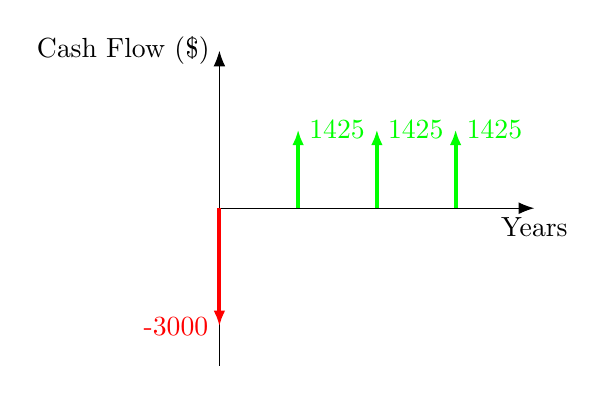
\begin{tikzpicture}[scale=1] \draw[-{Latex[length=2mm]}] (0,0) -- (4,0) node[anchor=north] {Years}; \draw[-{Latex[length=2mm]}] (0,-2) -- (0,2) node[anchor=east] {Cash Flow (\$)}; \draw[red, line width=0.5mm, -{Latex[length=2mm]}] (0,0) -- (0,-1.5) node[anchor=east] {-3000}; \foreach \x in {1,2,3} { \draw[green, line width=0.5mm, -{Latex[length=2mm]}] (\x,0) -- (\x,1) node[anchor=west] {1425}; }\end{tikzpicture}}
\qquad
\subfloat[]{%
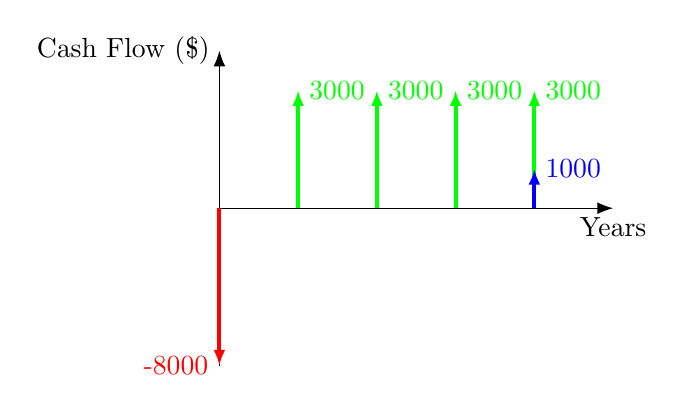
\begin{tikzpicture}[scale=1] \draw[-{Latex[length=2mm]}] (0,0) -- (5,0) node[anchor=north] {Years}; \draw[-{Latex[length=2mm]}] (0,-2) -- (0,2) node[anchor=east] {Cash Flow (\$)}; \draw[red, line width=0.5mm, -{Latex[length=2mm]}] (0,0) -- (0,-2) node[anchor=east] {-8000}; \foreach \x in {1,2,3,4} { \draw[green, line width=0.5mm, -{Latex[length=2mm]}] (\x,0) -- (\x,1.5) node[anchor=west] {3000}; } \draw[blue, line width=0.5mm, -{Latex[length=2mm]}] (4,0) -- (4,0.5) node[anchor=west] {1000};\end{tikzpicture}}
\qquad
\centering
\subfloat[]{%
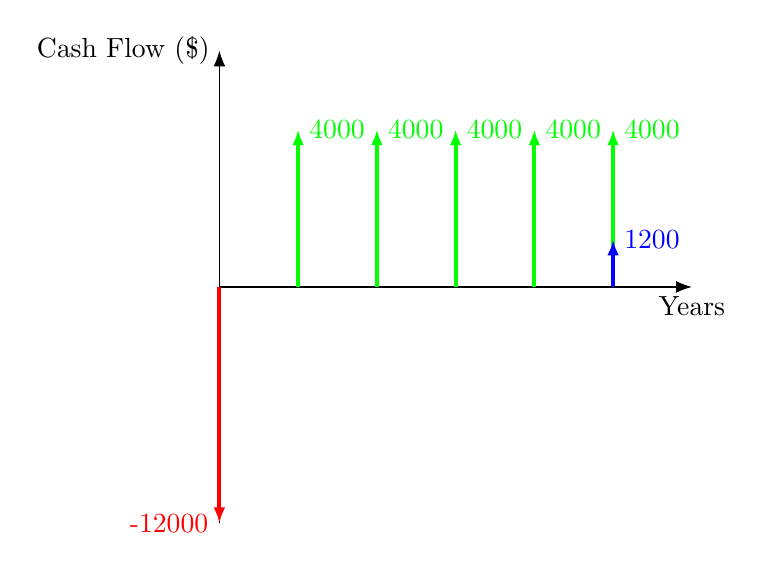
\begin{tikzpicture}[scale=1] \draw[-{Latex[length=2mm]}] (0,0) -- (6,0) node[anchor=north] {Years}; \draw[-{Latex[length=2mm]}] (0,-3) -- (0,3) node[anchor=east] {Cash Flow (\$)}; \draw[red, line width=0.5mm, -{Latex[length=2mm]}] (0,0) -- (0,-3) node[anchor=east] {-12000}; \foreach \x in {1,2,3,4,5} { \draw[green, line width=0.5mm, -{Latex[length=2mm]}] (\x,0) -- (\x,2) node[anchor=west] {4000}; } \draw[blue, line width=0.5mm, -{Latex[length=2mm]}] (5,0) -- (5,0.6) node[anchor=west] {1200}; \end{tikzpicture}}
\end{adjustwidth}
\end{figure}


\begin{figure}[!ht]
    \centering
    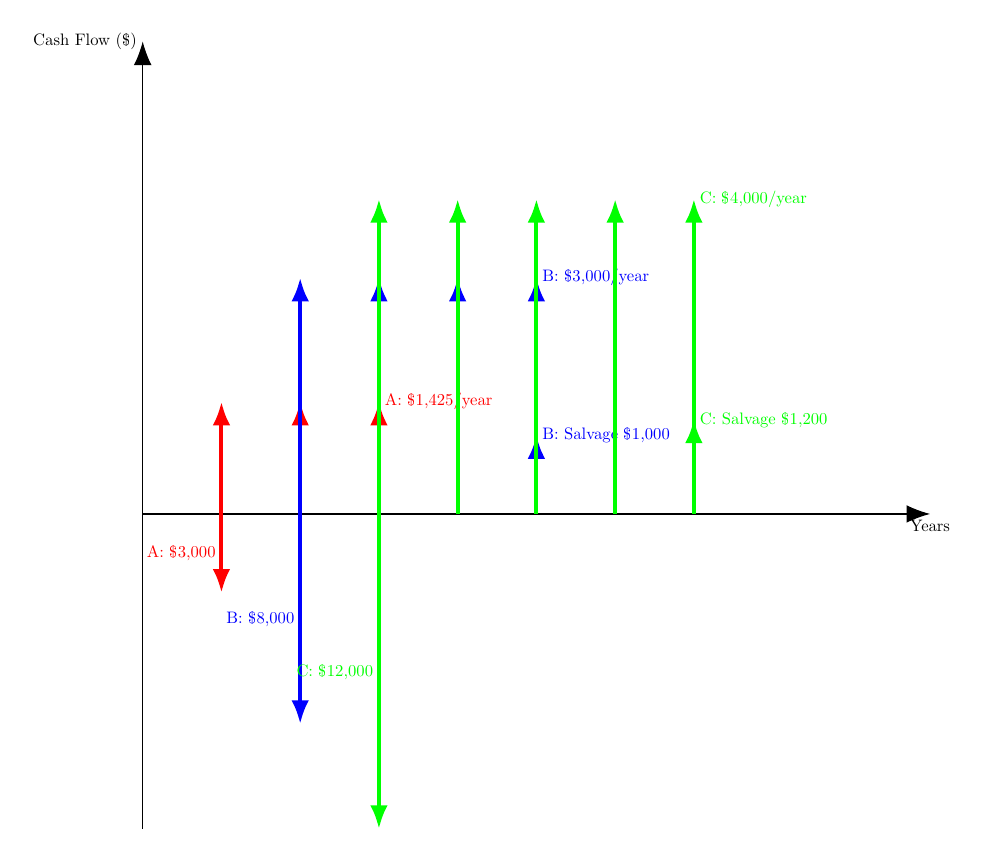
\begin{tikzpicture}[scale=1, every node/.style={scale=0.6}]
        % Draw axes
        \draw[-{Latex[length=3mm]}] (0,0) -- (10,0) node[anchor=north] {Years};
        \draw[-{Latex[length=3mm]}] (0,-4) -- (0,6) node[anchor=east] {Cash Flow (\$)};

        % Option A
        \draw[red, line width=0.5mm, -{Latex[length=3mm]}] (1,0) -- (1,-1);
        \foreach \y in {1,2,3} {
            \draw[red, line width=0.5mm, -{Latex[length=3mm]}] (\y,0) -- (\y,1.425);
        }
        \node[red, anchor=east] at (1, -1.5/3) {A: \$3,000};
        \node[red, anchor=west] at (3, 1.425) {A: \$1,425/year};

        % Option B
        \draw[blue, line width=0.5mm, -{Latex[length=3mm]}] (2,0) -- (2,-8/3);
        \foreach \y in {1,2,3,4} {
            \draw[blue, line width=0.5mm, -{Latex[length=3mm]}] (\y+1,0) -- (\y+1,3);
        }
        \draw[blue, line width=0.5mm, -{Latex[length=3mm]}] (5,0) -- (5,1);
        \node[blue, anchor=east] at (2, -4/3) {B: \$8,000};
        \node[blue, anchor=west] at (5, 3) {B: \$3,000/year};
        \node[blue, anchor=west] at (5, 1) {B: Salvage \$1,000};

        % Option C
        \draw[green, line width=0.5mm, -{Latex[length=3mm]}] (3,0) -- (3,-4);
        \foreach \y in {1,2,3,4,5} {
            \draw[green, line width=0.5mm, -{Latex[length=3mm]}] (\y+2,0) -- (\y+2,4);
        }
        \draw[green, line width=0.5mm, -{Latex[length=3mm]}] (7,0) -- (7,1.2);
        \node[green, anchor=east] at (3, -6/3) {C: \$12,000};
        \node[green, anchor=west] at (7, 4) {C: \$4,000/year};
        \node[green, anchor=west] at (7, 1.2) {C: Salvage \$1,200};

    \end{tikzpicture}
    \caption{Cash flow diagram for home painting business options.}
    \label{fig:painting-business-options}
\end{figure}

\newpage

Substituting the given values, we compute the NPVs for each option:

\textbf{Option A:}
\[
\begin{aligned}
I_A &= \$3,000, \ R_{A,t} = \$1,425 \ \forall t \in \{1, 2, 3\}, \ S_A = \$0, \ n_A = 3, \\
\text{NPV}_A &= -\$3,000 + \sum_{t=1}^{3} \frac{\$1,425}{(1 + 0.08)^t} \approx \$672.36.
\end{aligned}
\]

\textbf{Option B:}
\[
\begin{aligned}
I_B &= \$8,000, \ R_{B,t} = \$3,000 \ \forall t \in \{1, 2, 3, 4\}, \ S_B = \$1,000, \ n_B = 4, \\
\text{NPV}_B &= -\$8,000 + \sum_{t=1}^{4} \frac{\$3,000}{(1 + 0.08)^t} + \frac{\$1,000}{(1 + 0.08)^4} \approx \$2671.41.
\end{aligned}
\]

\textbf{Option C:}
\[
\begin{aligned}
I_C &= \$12,000, \ R_{C,t} = \$4,000 \ \forall t \in \{1, 2, 3, 4, 5\}, \ S_C = \$1,200, \ n_C = 5, \\
\text{NPV}_C &= -\$12,000 + \sum_{t=1}^{5} \frac{\$4,000}{(1 + 0.08)^t} + \frac{\$1,200}{(1 + 0.08)^5} \approx \$4787.54.
\end{aligned}
\]

\(\therefore \) For part \(a\), all options are financially acceptable as \(\text{NPV}_X > 0\) for each \(X \in \mathcal{O}\). For part \(b\), I am assuming that



\begin{table}[!ht]
\centering
\label{tab:my_label}
\resizebox{\textwidth}{!}{
\begin{tabular}{|c|c|}

\hline
\textbf{Condition/Assumption} & \textbf{Description} \\
\hline

\text{Consistent Cash Flow Sign} &
   $\forall f \in \mathcal{F}, \exists s \in \{-1, 1\} : \forall t \in \mathbb{N}, f(t) \cdot s \geq 0$ \\
\hline

\text{Predictable Cash Flows} & $\forall f \in \mathcal{F}, \exists \epsilon > 0 : \forall t \in \mathbb{N}, |f(t) - \hat{f}(t)| < \epsilon$ \\
\hline

\text{Stable Investment Environment} & $\nexists t \in \mathbb{N} : \Delta E(t) > \theta$ \\
\hline

\text{Fixed MARR} & $\forall t_1, t_2 \in \mathbb{N}, t_1 \neq t_2 : r_{\text{MARR}}(t_1) = r_{\text{MARR}}(t_2)$ \\
\hline

\text{Reinvestment Rate Assumption} & $\forall f \in \mathcal{F}, t \in \mathbb{N} : \text{Reinvest}(f(t)) = f(t) \cdot (1 + r_{\text{IRR}})$ \\
\hline

\text{Solvable IRR Equation} & $\exists! r_{\text{IRR}} \in \mathbb{R} : -I + \sum_{t=1}^{n} \frac{f(t)}{(1 + r_{\text{IRR}})^t} = 0$ \\
\hline

\text{Independent Projects} &  $\forall f, g \in \mathcal{F}, f \neq g : \nexists t \in \mathbb{N} : f(t) \cap g(t) \neq \varnothing $\\
\hline

\text{Single IRR Solution} & $\forall f \in \mathcal{F} : \text{Count}(\{r_{\text{IRR}} \in \mathbb{R} : -I + \sum_{t=1}^{n} \frac{f(t)}{(1 + r_{\text{IRR}})^t} = 0\}) = 1 $\\
\hline
\end{tabular}
}
\caption{Assumptions for applying the method. Here, \(\hat{f}(t)\) represents an estimate of the cash flow at time \(t\), \(\Delta E(t)\) denotes a change in the external investment environment at time \(t\), and \(\theta\) is a threshold beyond which the stability assumption is violated.}
\end{table}

The optimal choice \(X^*\) is the one that satisfies:

\[
X^* = \underset{X \in \mathcal{O}}{\mathrm{argmax}} \ (\text{NPV}_X) \quad \text{subject to} \quad r_X \geq r_{\text{MARR}}
\]

\(\therefore \) According to the yearly Worth and Decision Criterion method, yields \(X^* = C\) is the best choice from a business point of view because it has the highest yearly value.

\subsubsection*{Extra Note for The Part Specified in The Solutions to The Past Questions "CE231 MT FALL 2021 - SOLQ4"}
\addcontentsline{toc}{subsection}{Extra Note}
\[
FW_{X, N=5} = -I_X + \sum_{t=1}^{\min(n_X, 5)} R_{X,t} \cdot (1 + r_{\text{MARR}})^{5-t} + \mathbb{1}_{\{n_X \geq 5\}} \cdot S_X \cdot (1 + r_{\text{MARR}})^{5-n_X}
\]

where \(\mathbb{1}_{\{n_X \geq 5\}}\) is the indicator function, equal to 1 if \(n_X \geq 5\) and 0 otherwise. For options A, B, and C, the calculations are:

\[
\begin{aligned}
FW_{A, N=5} &= -\$3,000 + \sum_{t=1}^{3} \$1,425 \cdot (1 + 0.08)^{5-t} \\
FW_{B, N=5} &= -\$8,000 + \sum_{t=1}^{4} \$3,000 \cdot (1 + 0.08)^{5-t} + \$1,000 \cdot (1 + 0.08)^{5-4} \\
FW_{C, N=5} &= -\$12,000 + \sum_{t=1}^{5} \$4,000 \cdot (1 + 0.08)^{5-t} + \$1,200 \cdot (1 + 0.08)^{5-5}
\end{aligned}
\]

Evaluating these expressions yields the future worths:

\[
\begin{aligned}
FW_{A, N=5} &= \$2,395.91 \\
FW_{B, N=5} &= \$6,599.80 \\
FW_{C, N=5} &= \$12,666.40
\end{aligned}
\]

Thus, according to the criterion of maximizing future worth at \(N = 5\), option \(C\) is selected.

\[
0 = -I_B + \sum_{t=1}^{n_B} \frac{R_{B,t}}{(1 + r_B)^t} + \frac{S_B}{(1 + r_B)^{n_B}}
\]

For Option B, \( I_B = \$8,000 \), \( R_{B,t} = \$3,000 \) for \( t = 1, 2, 3, 4 \), and \( S_B = \$1,000 \). Substituting these values, the equation becomes:

\[
0 = -\$8,000 + \frac{\$3,000}{(1 + r_B)} + \frac{\$3,000}{(1 + r_B)^2} + \frac{\$3,000}{(1 + r_B)^3} + \frac{\$4,000}{(1 + r_B)^4} \implies \$ 3000 \frac{1-(1+r_B)^{-4}}{r_B}=\$8000
\]

Using mathematica (\href{https://www.wolframalpha.com/input?i=0+%3D+-8000+%2B+3000%2F%281+%2B+r%29+%2B+3000%2F%281+%2B+r%29%5E2+%2B+3000%2F%281+%2B+r%29%5E3+%2B+%283000+%2B+1000%29%2F%281+%2B+r%29%5E4}{\textcolor{red}{ WolframAlpha Code Here}}) command gives

\[\{r\to 0.215608\}\]

For the investment to be deemed feasible, it must hold that \( r_B \geq r_{\text{MARR}} \). Given \( r_{\text{MARR}} = 8\% \), The Internal Rate of Return (IRR) for Option B is approximately \(21.56\%\). Since this IRR is greater than the Minimum Attractive Rate of Return (MARR) of \(8\%\), \(\therefore \) Option B is financially feasible according to this criterion. 

\subsubsection*{Summary}
\addcontentsline{toc}{subsection}{Summary}
\[
\resizebox{\textwidth}{!}{
\begin{array}{|c|c|}
\hline
\text{Part} & \text{Solution} \\
\hline
(a) & \begin{aligned} 
\text{Let } & \text{NPV}_X = -I_X + \sum_{t=1}^{n_X} \frac{R_{X,t}}{(1 + r_{\text{MARR}})^t} + \frac{S_X}{(1 + r_{\text{MARR}})^{n_X}}, \\
\text{where} & \ I_X, R_{X,t}, S_X, n_X \text{ are initial investment, net annual revenue,} \\
& \text{salvage value, and useful life of capital for option } X, \text{ respectively, and } \\
& \ r_{\text{MARR}} = 0.08. \\
\text{Then} & \ \text{NPV}_A \approx 672.36, \ \text{NPV}_B \approx 2671.41, \ \text{NPV}_C \approx 4787.54, \\
\text{Thus} & \ \{A, B, C\} \text{ are financially acceptable (NPVs are positive)}. 
\end{aligned} \\
\hline
(b) & \begin{aligned} 
\text{Maximize} & \ \text{NPV}_X \text{ subject to } r_X \geq r_{\text{MARR}}, \\
\text{Yields} & \ X^* = C \ (\text{as } \text{NPV}_C \text{ is maximal}). 
\end{aligned} \\
\hline
(c) & \begin{aligned} 
\text{Solve} & \ 0 = -I_B + \sum_{t=1}^{n_B} \frac{R_{B,t}}{(1 + r_B)^t} + \frac{S_B}{(1 + r_B)^{n_B}} \text{ for } r_B, \\
\text{Gives} & \ r_B \approx 21.56\%, \\
\text{As} & \ r_B > r_{\text{MARR}}, \text{ Option B is feasible}. 
\end{aligned} \\
\hline
\end{array}
}
\]

\newpage
\subsection*{Question 4-80}
\addcontentsline{toc}{section}{Question 4-80}
\begin{q}
Calculate the future equivalent at the end of 2012, at \(8 \%\) per year, of the following series of cash flows in Figure P4-80: [Use a uniform gradient amount \((G)\) in your solution.] (4.11)
\end{q}

\begin{figure}[!ht]
    \centering
    \begin{tikzpicture}[scale=1.4, every node/.style={scale=1}]
        % Draw axes
        \draw[-{Latex[length=3mm]}] (0,0) -- (6,0) node[anchor=north] {Year};
        \draw[-{Latex[length=3mm]}] (0,-3) -- (0,3) node[anchor=east] {Cash Flow (\$)};

        % Define years
        \foreach \x/\year in {1/2009, 2/2010, 3/2011, 4/2012, 5/2013} {
            \draw (\x,3pt) -- (\x,-3pt) node[anchor=north] {\year};
        }

        % Cash flows
        \draw[red, line width=0.5mm, -{Latex[length=3mm]}] (1,0) -- (1,-2) node[anchor=east] {\$1000};
        \draw[red, line width=0.5mm, -{Latex[length=3mm]}] (2,0) -- (2,-1.6) node[anchor=east] {\$800};
        \draw[red, line width=0.5mm, -{Latex[length=3mm]}] (3,0) -- (3,-1.2) node[anchor=east] {\$600};
        \draw[red, line width=0.5mm, -{Latex[length=3mm]}] (4,0) -- (4,-0.8) node[anchor=east] {\$400};
        \draw[blue, line width=0.5mm, -{Latex[length=3mm]}] (5,0) -- (5,-3) node[anchor=west] {\$F};

    \end{tikzpicture}
    \caption{Cash flow diagram for the given problem, showing a series of decreasing payments from 2009 to 2012 and the future equivalent in 2013.}
    \label{fig:cash-flow}
\end{figure}

Let \( A \) be the initial annual cash flow, \( G \) the uniform gradient amount by which the cash flow decreases each year, \( i \) the interest rate per period, and \( N \) the total number of periods. For our specific problem, \( A = 1000 \), \( G = 200 \), \( i = 0.08 \), and \( N = 4 \).

\[ P1 = A \times \left(\frac{1 - (1 + i)^{-N}}{i}\right) = 1000 \times \left(\frac{1 - (1 + 0.08)^{-4}}{0.08}\right) = 3312.1268 \]
\[ P2 = G \times \left(\frac{\frac{1 - (1 + i)^{-N}}{i} - N \cdot (1 + i)^{-N}}{i}\right) = 200 \times \left(\frac{\frac{1 - (1 + 0.08)^{-4}}{0.08} - 4 \cdot (1 + 0.08)^{-4}}{0.08}\right) = 930.0186\]
\[P=P1 - P2 = 2382.1083 \]
\[\therefore F = P\times F_P = P (1 + i)^{N^\prime} = 2382.1083 (1+0.08)^5 =\boxed{3500.09856}. \]

\newpage
\subsection*{Question 5-39}
\addcontentsline{toc}{section}{Question 5-39}
\begin{q}
A large lithium-ion phosphate battery pack for an industrial application is expected to save \(\$ 20,000\) in annual energy expenses over its 6-year life. For a 3-year simple payback period, the permissible capital investment is \(\$ 60,000\). What is the internal rate of return on this \(\$ 60,000\) battery pack if it has a residual value of \(\$ 10,000\) at the end of 6 years? The MARR is \(18 \%\) per year. (5.6)
\end{q}


\begin{figure}[!ht]
    \centering
    \begin{tikzpicture}[scale=1.2, every node/.style={scale=0.8}]
        % Draw axes
        \draw[-{Latex[length=3mm]}] (0,0) -- (9,0) node[anchor=north] {Years};
        \draw[-{Latex[length=3mm]}] (0,-4.5) -- (0,4.5) node[anchor=east] {Cash Flow (\$)};

        % Initial investment
        \draw[red, line width=0.5mm, -{Latex[length=3mm]}] (1,0) -- (1,-6/2);
        \node[red, anchor=east] at (1, -3/2) {Investment \$60,000};

        % Annual savings
        \foreach \y in {1,2,3,4,5,6} {
            \draw[blue, line width=0.5mm, -{Latex[length=3mm]}] (\y+1,0) -- (\y+1,3.3/2);
            \node[blue, anchor=west] at (\y+1, 1.65/2) {\$20,000};
        }

        % Residual value
        \draw[green, line width=0.5mm, -{Latex[length=3mm]}] (7,0) -- (7,2/2);
        \node[green, anchor=west] at (7, 1/2.5) {Residual \$10,000};

    \end{tikzpicture}
    \caption{Cash flow diagram for the investment in a lithium-ion phosphate battery pack.}
    \label{fig:battery-pack-investment}
\end{figure}

Here
\[
0 = -60,000 + \sum_{t=1}^{6} \frac{20,000}{(1 + r)^t} + \frac{10,000}{(1 + r)^6}.
\]

Thus (\href{https://www.wolframalpha.com/input?i=60000+-+10000%2F%281%2Br%29%5E6%3D+sum+20000%2F%281%2Br%29%5Et+from+t%3D1+to+6}{\textcolor{red}{WolframAlpha}})
\[\therefore \boxed{r = 0.2614 \quad (26.15 \%)}.\]

\newpage
\subsection*{Question 6-28}
\addcontentsline{toc}{section}{Question 6-28}
\begin{q}
Consider the following EOY cash flows for two mutually exclusive alternatives (one must be chosen):
\begin{center}
\begin{tabular}{llc}
\hline & Lead Acid & Lithium Ion \\
\hline Capital investment & \(\$ 6,000\) & \(\$ 14,000\) \\
Annual expenses & \(\$ 2,500\) & \(\$ 2,400\) \\
Useful life & 12 years & 18 years \\
Market value at & \(\$ 0\) & \(\$ 2,800\) \\
\(\quad\) end of useful life & & \\
\hline
\end{tabular}
\end{center}
The MARR is \(5 \%\) per year. (6.5)

a. Determine which alternative should be selected if the repeatability assumption applies.

b. Determine which alternative should be selected if the analysis period is 18 years, the repeatability assumption does not apply, and a battery system can be leased for \(\$ 8,000\) per year after the useful life of either battery is over.
\end{q}


\begin{figure}[!ht]
    \centering
    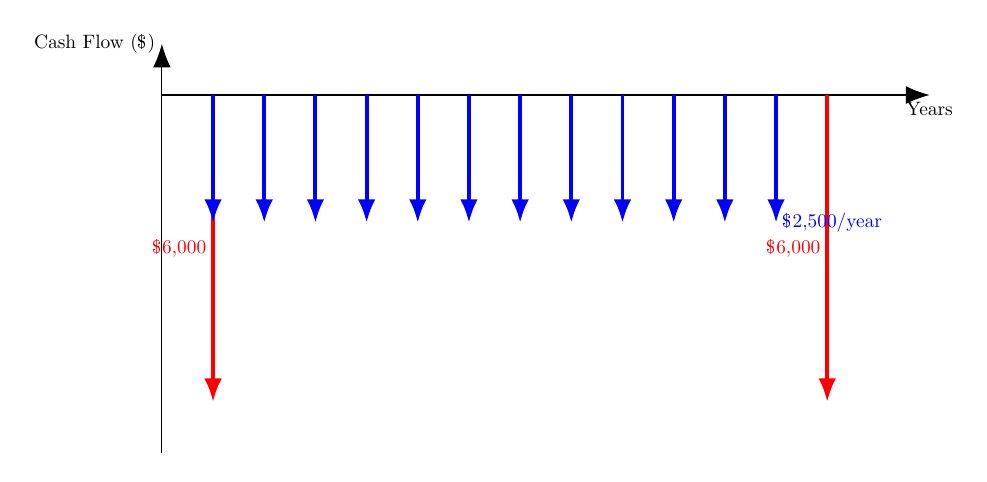
\begin{tikzpicture}[scale=0.65, every node/.style={scale=0.7}]
        % Draw axes
        \draw[-{Latex[length=3mm]}] (0,0) -- (15,0) node[anchor=north] {Years};
        \draw[-{Latex[length=3mm]}] (0,-7) -- (0,1) node[anchor=east] {Cash Flow (\$)};

        % Initial investment
        \draw[red, line width=0.5mm, -{Latex[length=3mm]}] (1,0) -- (1,-6);
        \node[red, anchor=east] at (1, -3) {\$6,000};

        % Annual expenses
        \foreach \y in {1,2,...,12} {
            \draw[blue, line width=0.5mm, -{Latex[length=3mm]}] (\y,0) -- (\y,-2.5);
        }

        % Replacement after 12 years
        \draw[red, line width=0.5mm, -{Latex[length=3mm]}] (13,0) -- (13,-6);
        \node[red, anchor=east] at (13, -3) {\$6,000};
        
        \node[blue, anchor=west] at (12, -2.5) {\$2,500/year};
    \end{tikzpicture}
    \caption{Cash flow diagram for Lead Acid battery over 18 years.}
    \label{fig:lead-acid-battery-cash-flow}
\end{figure}


\begin{figure}[!ht]
    \centering
    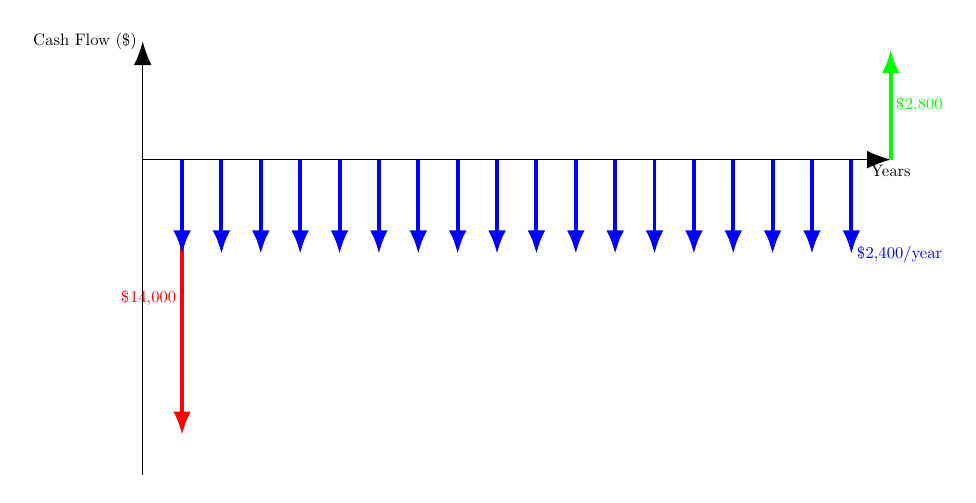
\begin{tikzpicture}[scale=0.5, every node/.style={scale=0.6}]
        % Draw axes
        \draw[-{Latex[length=3mm]}] (0,0) -- (19,0) node[anchor=north] {Years};
        \draw[-{Latex[length=3mm]}] (0,-8) -- (0,3) node[anchor=east] {Cash Flow (\$)};

        % Initial investment
        \draw[red, line width=0.5mm, -{Latex[length=3mm]}] (1,0) -- (1,-7);
        \node[red, anchor=east] at (1, -3.5) {\$14,000};

        % Annual expenses
        \foreach \y in {1,2,...,18} {
            \draw[blue, line width=0.5mm, -{Latex[length=3mm]}] (\y,0) -- (\y,-2.4);
        }

        % Market value at end of useful life
        \draw[green, line width=0.5mm, -{Latex[length=3mm]}] (19,0) -- (19,2.8);
        \node[green, anchor=west] at (19, 1.4) {\$2,800};

        \node[blue, anchor=west] at (18, -2.4) {\$2,400/year};
    \end{tikzpicture}
    \caption{Cash flow diagram for Lithium Ion battery over 18 years.}
    \label{fig:lithium-ion-battery-cash-flow}
\end{figure}
\newpage

Let \( C_0^{(L)} \) and \( C_0^{(I)} \) be the initial capital investments for Lead Acid and Lithium Ion, respectively, where \( C_0^{(L)} = -\$6,000 \) and \( C_0^{(I)} = -\$14,000 \). The annual expenses, \( A^{(L)} \) and \( A^{(I)} \), are \( -\$2,500 \) and \( -\$2,400 \) for Lead Acid and Lithium Ion, respectively. The respective useful lives \( n^{(L)} \) and \( n^{(I)} \) are 12 and 18 years. The market values at the end of the useful life, \( S_n^{(L)} \) and \( S_n^{(I)} \), are \( \$0 \) and \( \$2,800 \) for Lead Acid and Lithium Ion, respectively. The Equivalent yearly Cost (EAC) is what makes the choice possible. It takes the present value of all the cash flows and turns them into a regular yearly series over the life of the project. For each alternative \( X \), the Present Worth (PW) is expressed as:

\[ \text{PW}^{(X)} = C_0^{(X)} + A^{(X)} \cdot \left( \frac{(1 + i)^{n^{(X)}} - 1}{i(1 + i)^{n^{(X)}}} \right) + S_n^{(X)} \cdot \left( \frac{1}{(1 + i)^{n^{(X)}}} \right). \]

The EAC is then:
\[ \text{EAC}^{(X)} = \text{PW}^{(X)} \cdot \left( \frac{i(1 + i)^{n^{(X)}}}{(1 + i)^{n^{(X)}} - 1} \right). \]

So

\[\text{EAC}^{(X)} = \Bigg[ C_0^{(X)} + A^{(X)} \cdot \left( \frac{(1 + i)^{n^{(X)}} - 1}{i(1 + i)^{n^{(X)}}} \right) + S_n^{(X)} \cdot \left( \frac{1}{(1 + i)^{n^{(X)}}} \right)\Bigg] \cdot \left( \frac{i(1 + i)^{n^{(X)}}}{(1 + i)^{n^{(X)}} - 1} \right). \]

We proceed to calculate the EAC for each alternative

\begin{figure}[!ht]
    \centering
    \includegraphics[width=\textwidth]{Screenshot 2023-11-26 201053.png}
    \caption{Mathematica Code}
    \label{fig:enter-label}
\end{figure}

\[\{-28158.1,-40891.6,-3176.95,-3498.12\}.\]

In this case, the Lead Acid alternative, with an EAC of \(-\$3,176.95\), is more economical compared to the Lithium Ion alternative, which has an EAC of \(-\$3,498.12\). Therefore, \(\therefore\)\textbf{the Lead Acid} alternative should be selected.

\newpage
\subsection*{Question 6-44}
\addcontentsline{toc}{section}{Question 6-44}
\begin{q}
Three mutually exclusive earth-moving pieces of equipment are being considered for several large building projects in India over the next five years. The estimated cash flows for each alternative are given below. The construction company's MARR is \(15 \%\) per year. Which of the three alternatives, if any, should be adopted? State your main assumptions. (6.5)
\begin{center}
\begin{tabular}{lrrr}
\hline & Caterpillar & Deere & \multicolumn{1}{c}{ Case } \\
\hline Capital investment & \(\$ 22,000\) & \(\$ 26,200\) & \(\$ 17,000\) \\
Net annual revenue & \(\$ 7,000\) & \(\$ 9,500\) & \(\$ 5,200\) \\
Salvage value & \(\$ 4,000\) & \(\$ 5,000\) & \(\$ 3,500\) \\
Useful life & 4 years & 3 years & 5 years \\
\hline
\end{tabular}
\end{center}
\end{q}




\begin{adjustwidth}{-2cm}{-2cm}
\begin{figure}[!ht]
    \centering
    \begin{minipage}[b]{0.32\textwidth}
        \flushleft
        % Caterpillar equipment cash flow diagram

        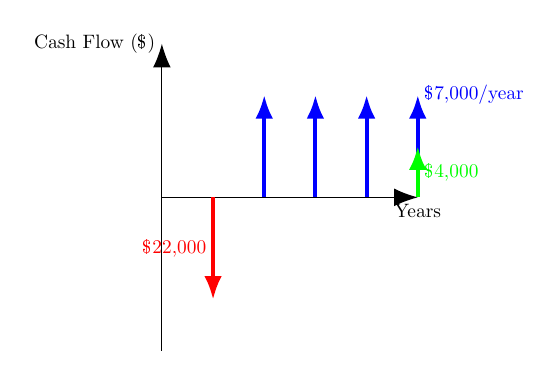
\begin{tikzpicture}[scale=0.65, every node/.style={scale=0.7}]
        % Draw axes
        \draw[-{Latex[length=3mm]}] (0,0) -- (5,0) node[anchor=north] {Years};
        \draw[-{Latex[length=3mm]}] (0,-3) -- (0,3) node[anchor=east] {Cash Flow (\$)};

        % Initial investment
        \draw[red, line width=0.5mm, -{Latex[length=3mm]}] (1,0) -- (1,-2);
        \node[red, anchor=east] at (1, -1) {\$22,000};

        % Net annual revenue
        \foreach \y in {1,2,3,4} {
            \draw[blue, line width=0.5mm, -{Latex[length=3mm]}] (\y+1,0) -- (\y+1,2);
        }

        % Salvage value
        \draw[green, line width=0.5mm, -{Latex[length=3mm]}] (5,0) -- (5,1);
        \node[green, anchor=west] at (5, 0.5) {\$4,000};

        \node[blue, anchor=west] at (5, 2) {\$7,000/year};
    \end{tikzpicture}
        \caption{Cash flow diagram for Caterpillar equipment.}
        \label{fig:caterpillar-equipment-cash-flow}
    \end{minipage}
    \begin{minipage}[b]{0.32\textwidth}
        \centering
        % Deere equipment cash flow diagram
        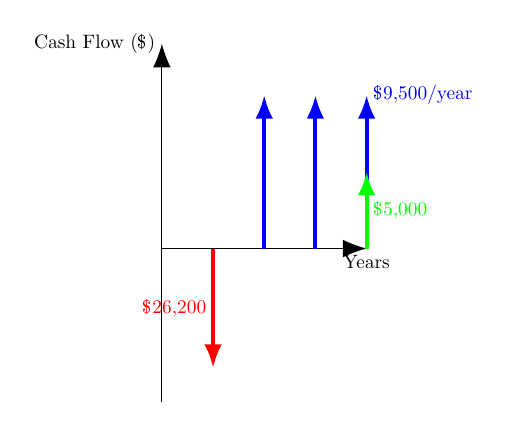
\begin{tikzpicture}[scale=0.65, every node/.style={scale=0.7}]
            % Draw axes
        \draw[-{Latex[length=3mm]}] (0,0) -- (4,0) node[anchor=north] {Years};
        \draw[-{Latex[length=3mm]}] (0,-3) -- (0,4) node[anchor=east] {Cash Flow (\$)};

        % Initial investment
        \draw[red, line width=0.5mm, -{Latex[length=3mm]}] (1,0) -- (1,-7/3);
        \node[red, anchor=east] at (1, -3.5/3) {\$26,200};

        % Net annual revenue
        \foreach \y in {1,2,3} {
            \draw[blue, line width=0.5mm, -{Latex[length=3mm]}] (\y+1,0) -- (\y+1,3);
        }

        % Salvage value
        \draw[green, line width=0.5mm, -{Latex[length=3mm]}] (4,0) -- (4,1.5);
        \node[green, anchor=west] at (4, 0.75) {\$5,000};

        \node[blue, anchor=west] at (4, 3) {\$9,500/year};
        \end{tikzpicture}
        \caption{Cash flow diagram for Deere equipment.}
        \label{fig:deere-equipment-cash-flow}
    \end{minipage}
    \begin{minipage}[b]{0.32\textwidth}
        \flushright
        % Case equipment cash flow diagram
        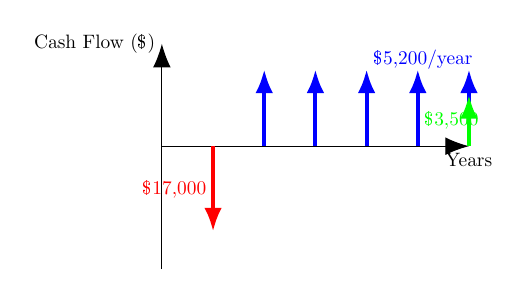
\begin{tikzpicture}[scale=0.65, every node/.style={scale=0.7}]
           % Draw axes
        \draw[-{Latex[length=3mm]}] (0,0) -- (6,0) node[anchor=north] {Years};
        \draw[-{Latex[length=3mm]}] (0,-6/2.5) -- (0,2) node[anchor=east] {Cash Flow (\$)};

        % Initial investment
        \draw[red, line width=0.5mm, -{Latex[length=3mm]}] (1,0) -- (1,-5/3);
        \node[red, anchor=east] at (1, -2.5/3) {\$17,000};

        % Net annual revenue
        \foreach \y in {1,2,3,4,5} {
            \draw[blue, line width=0.5mm, -{Latex[length=3mm]}] (\y+1,0) -- (\y+1,1.5);
        }

        % Salvage value
        \draw[green, line width=0.5mm, -{Latex[length=3mm]}] (6,0) -- (6,1);
        \node[green, anchor=west] at (5, 0.5) {\$3,500};

        \node[blue, anchor=west] at (4, 1.7) {\$5,200/year};
        \end{tikzpicture}
        \caption{Cash flow diagram for Case equipment.}
        \label{fig:case-equipment-cash-flow}
    \end{minipage}
\end{figure}
\end{adjustwidth}











\begin{table}[h]
\centering
\resizebox{\textwidth}{!}{
\[
\begin{array}{|c|c|}
\hline
\textbf{Condition/Assumption} & \textbf{Description} \\
\hline
\text{Initial Investment Outflow} & \forall j \in \{ \text{Caterpillar, Deere, Case} \}, C_{0,j} < 0 \\
\hline
\text{Constant Annual Revenue} & \forall j \in \{ \text{Caterpillar, Deere, Case} \}, \exists R_j \in \mathbb{R} : \forall t \in \{1, \ldots, n_j\}, R_{t,j} = R_j \\
\hline
\text{Determinate Salvage Value} & \forall j \in \{ \text{Caterpillar, Deere, Case} \}, \exists S_{n_j,j} \in \mathbb{R} \\
\hline
\text{Fixed MARR} & \forall t_1, t_2 \in \mathbb{N}, t_1 \neq t_2 : i(t_1) = i(t_2) = 0.15 \\
\hline
\text{Discounted Cash Flow Principle} & \forall j \in \{ \text{Caterpillar, Deere, Case} \}, \forall t \in \{1, \ldots, n_j\} : \frac{R_{t,j}}{(1 + i)^t} \\
\hline
\text{Mutual Exclusivity of Projects} & \forall j, k \in \{ \text{Caterpillar, Deere, Case} \}, j \neq k : \text{Selection of } j \implies \text{Non-selection of } k \\
\hline
\text{Time-Bounded Project Life} & \forall j \in \{ \text{Caterpillar, Deere, Case} \}, \exists n_j \in \mathbb{N} \\
\hline
\text{No Interim Salvage Value} & \forall j \in \{ \text{Caterpillar, Deere, Case} \}, \forall t < n_j : S_{t,j} = 0 \\
\hline
\end{array}
\]
}
\caption{Assumptions and Conditions for Q6-44}
\label{table:investment_analysis}
\end{table}



The general formulation for the PW

\[
PW = -C_0 + \sum_{t=1}^{n} \frac{R_t}{(1 + i)^t} + \frac{S_n}{(1 + i)^n},
\]

where \( C_0 \) represents the initial capital investment, \( R_t \) is the net annual revenue in year \( t \), \( S_n \) denotes the salvage value at the end of year \( n \), and \( n \) is the useful life of the equipment in years.


\subsubsection*{Caterpillar}
Let \( C_0 = -\$22,000 \), \( R_t = \$7,000 \) for \( t = 1, \ldots, 4 \), \( S_4 = \$4,000 \), and \( n = 4 \). Then, the PW for Caterpillar is given by:

\[
PW_{\text{Caterpillar}} = -22,000 + \sum_{t=1}^{4} \frac{7,000}{(1 + 0.15)^t} + \frac{4,000}{(1 + 0.15)^4} = \$271.86.
\]

\subsubsection*{Deere}
Let \( C_0 = -\$26,200 \), \( R_t = \$9,500 \) for \( t = 1, \ldots, 3 \), \( S_3 = \$5,000 \), and \( n = 3 \). Then, the PW for Deere is given by:

\[
PW_{\text{Deere}} = -26,200 + \sum_{t=1}^{3} \frac{9,500}{(1 + 0.15)^t} + \frac{5,000}{(1 + 0.15)^3} = -\$1,221.78.
\]

\subsubsection*{Case}
Let \( C_0 = -\$17,000 \), \( R_t = \$5,200 \) for \( t = 1, \ldots, 5 \), \( S_5 = \$3,500 \), and \( n = 5 \). Then, the PW for Case is given by:

\[
PW_{\text{Case}} = -17,000 + \sum_{t=1}^{5} \frac{5,200}{(1 + 0.15)^t} + \frac{3,500}{(1 + 0.15)^5} = \$2,171.33.
\]

Based on these numbers, the \(\therefore\)\textbf{Case} equipment is the best choice from a business point of view since it has the biggest positive present value.


\newpage
\subsection*{Question 6-81}
\addcontentsline{toc}{section}{Question 6-81}
\begin{q}
For the following table, assume a MARR of \(15 \%\) per year and a useful life for each alternative of eight years which equals the study period. The rank-order of alternatives from least capital investment to greatest capital investment is \(Z \rightarrow Y \rightarrow W \rightarrow X\). Complete the incremental analysis by selecting the preferred alternative. "Do nothing" is not an option. (6.4)

\begin{center}
\begin{tabular}{cccc}
\hline & \(Z \rightarrow Y\) & \(Y \rightarrow W\) & \(W \rightarrow X\) \\
\hline\(\Delta\) Capital & \(-\$ 250\) & \(-\$ 400\) & \(-\$ 550\) \\
\begin{tabular}{c} 
investment \\
\(\Delta\) Annual cost \\
savings
\end{tabular} & 70 & 90 & 15 \\
\begin{tabular}{c}
\(\Delta\) Market \\
value
\end{tabular} & 100 & 50 & 200 \\
\(\Delta\) PW(15\%) & 97 & 20 & \(? ? ?\) \\
\hline
\end{tabular}
\end{center}
\end{q}



\begin{figure}[!ht]
    \centering
    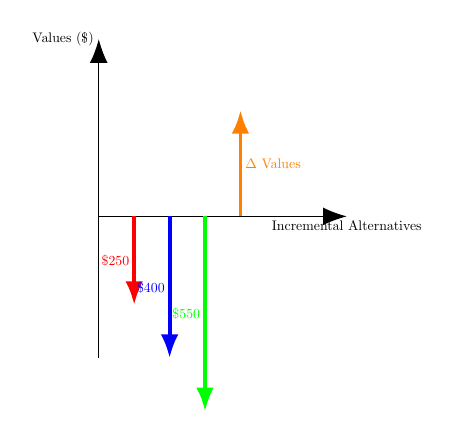
\begin{tikzpicture}[scale=0.45, every node/.style={scale=0.5}]
        % Draw axes
        \draw[-{Latex[length=3mm]}] (0,0) -- (7,0) node[anchor=north] {Incremental Alternatives};
        \draw[-{Latex[length=3mm]}] (0,-4) -- (0,5) node[anchor=east] {Values (\$)};

        % Z to Y
        \draw[red, line width=0.5mm, -{Latex[length=3mm]}] (1,0) -- (1,-2.5);
        \node[red, anchor=east] at (1, -1.25) {\(\$250\)};

        % Y to W
        \draw[blue, line width=0.5mm, -{Latex[length=3mm]}] (2,0) -- (2,-4);
        \node[blue, anchor=east] at (2, -2) {\(\$400\)};

        % W to X
        \draw[green, line width=0.5mm, -{Latex[length=3mm]}] (3,0) -- (3,-5.5);
        \node[green, anchor=east] at (3, -2.75) {\(\$550\)};

        % Delta Annual Cost Savings and Market Value (approximated)
        \draw[orange, line width=0.5mm, -{Latex[length=3mm]}] (4,0) -- (4,3);
        \node[orange, anchor=west] at (4, 1.5) {\(\Delta\) Values};


    \end{tikzpicture}
    \caption{Cash Flow Diagram for The Incremental Analysis Cash Flow Q6-81}
    \label{fig:incremental-analysis-cash-flow}
\end{figure}

Let \(\Delta \text{Capital}_{ij}\) be the change in capital investment, \(\Delta \text{AC}_{ij}\) the annual cost savings, and \(\Delta \text{MV}_{ij}\) the market value at the conclusion of the project lifecycle, for each transition \(i \rightarrow j\). The present worth \(\Delta \text{PW}_{ij}\) is then:

\[
\Delta \text{PW}_{ij} = -\Delta \text{Capital}_{ij} + \sum_{t=1}^{n} \frac{\Delta \text{AC}_{ij}}{(1 + r)^t} + \frac{\Delta \text{MV}_{ij}}{(1 + r)^n},
\]

where \(r\) is the MARR, and \(n\) is the project duration. In the specific case of \(W \rightarrow X\), we have \(\Delta \text{Capital}_{WX} = -550\), \(\Delta \text{AC}_{WX} = 15\), and \(\Delta \text{MV}_{WX} = 200\). Yields:

\[
\Delta \text{PW}_{WX} = -550 + \sum_{t=1}^{8} \frac{15}{(1 + 0.15)^t} + \frac{200}{(1 + 0.15)^8} \approx -\$417.3098.
\]

Therefore, the preferred alternative among \(Z\), \(Y\), \(W\), and \(X\) is \(W\), becaude it offers the highest positive incremental PW without leading to a negative PW in the subsequent step.


\newpage
\subsection*{Question 6-84--6-85}
\addcontentsline{toc}{section}{Question 6-84 and 6-85}
\begin{q}
\textbf{6-84}. The IRR for Alternative \(A\) is most nearly:
(a) \(30 \%\) (b) \(15 \%\) (c) \(36 \%\) (d) \(10 \%\) (e) \(20 \%\)

\textbf{6-85}. Using a MARR of \(15 \%\), the preferred Alternative is:
(a) Do nothing (b) Alt. \(A\) (c) Alt. \(B\) (d) Alt. C (e) Alt. \(D\) (f) Alt. \(E\)
\vspace{0.5cm}

\resizebox{\textwidth}{!}{
\begin{tabular}{cccccc}
\hline
\multicolumn{7}{l}{ TABLE P6-82 } & Data for Problems 6-82 through 6-85 \\
\hline
& \(A\) & \multicolumn{1}{c}{ B } & \multicolumn{1}{c}{ C } & \multicolumn{1}{c}{ D } & \multicolumn{1}{c}{\(E\)} \\
\hline Capital investment & \(\$ 60,000\) & \(\$ 90,000\) & \(\$ 40,000\) & \(\$ 30,000\) & \(\$ 70,000\) \\
Annual expenses & 30,000 & 40,000 & 25,000 & 15,000 & 35,000 \\
Annual revenues & 50,000 & 52,000 & 38,000 & 28,000 & 45,000 \\
Market value at EOY 10 & 10,000 & 15,000 & 10,000 & 10,000 & 15,000 \\
IRR & \(? ? ?\) & \(7.4 \%\) & \(30.8 \%\) & \(42.5 \%\) & \(9.2 \%\) \\
\hline
\end{tabular}
}
\end{q}

\begin{figure}[!ht]
    \centering
    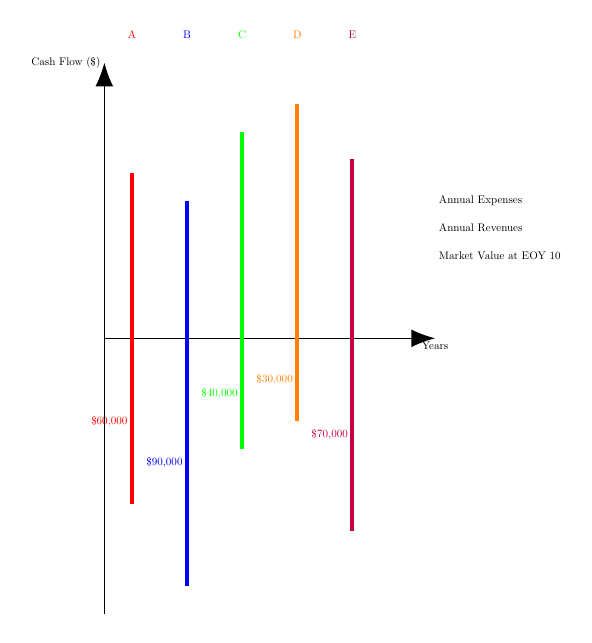
\begin{tikzpicture}[scale=0.35, every node/.style={scale=0.4}]
        % Draw axes
        \draw[-{Latex[length=3mm]}] (0,0) -- (12,0) node[anchor=north] {Years};
        \draw[-{Latex[length=3mm]}] (0,-10) -- (0,10) node[anchor=east] {Cash Flow (\$)};

        % Define positions for alternatives
        \def\A{1}
        \def\B{3}
        \def\C{5}
        \def\D{7}
        \def\E{9}

        % Alternative A
        \draw[red, line width=0.5mm] (\A, 0) -- (\A, -6) node[midway, left] {\$60,000};
        \foreach \y in {1,...,10} {
            \draw[red, line width=0.5mm] (\A, \y - 5) -- (\A, \y - 4);
        }
        \node[red] at (\A, 11) {A};

        % Alternative B
        \draw[blue, line width=0.5mm] (\B, 0) -- (\B, -9) node[midway, left] {\$90,000};
        \foreach \y in {1,...,10} {
            \draw[blue, line width=0.5mm] (\B, \y - 6) -- (\B, \y - 5);
        }
        \node[blue] at (\B, 11) {B};

        % Alternative C
        \draw[green, line width=0.5mm] (\C, 0) -- (\C, -4) node[midway, left] {\$40,000};
        \foreach \y in {1,...,10} {
            \draw[green, line width=0.5mm] (\C, \y - 3.5) -- (\C, \y - 2.5);
        }
        \node[green] at (\C, 11) {C};

        % Alternative D
        \draw[orange, line width=0.5mm] (\D, 0) -- (\D, -3) node[midway, left] {\$30,000};
        \foreach \y in {1,...,10} {
            \draw[orange, line width=0.5mm] (\D, \y - 2.5) -- (\D, \y - 1.5);
        }
        \node[orange] at (\D, 11) {D};

        % Alternative E
        \draw[purple, line width=0.5mm] (\E, 0) -- (\E, -7) node[midway, left] {\$70,000};
        \foreach \y in {1,...,10} {
            \draw[purple, line width=0.5mm] (\E, \y - 4.5) -- (\E, \y - 3.5);
        }
        \node[purple] at (\E, 11) {E};

        % Legend for annual expenses and revenues
        \node[anchor=west] at (12, 5) {Annual Expenses};
        \node[anchor=west] at (12, 4) {Annual Revenues};
        \node[anchor=west] at (12, 3) {Market Value at EOY 10};
    \end{tikzpicture}
    \caption{Cash Flow Diagram for Alternatives A, B, C, D, and E}
    \label{fig:alternatives-cash-flow}
\end{figure}

\[ \text{NPV}(r) = -C_0 + \sum_{t=1}^{n} \frac{R_t - E_t}{(1 + r)^t} + \frac{M_n}{(1 + r)^n}; \]

\[ -60,000 + \sum_{t=1}^{10} \frac{50,000 - 30,000}{(1 + r_A)^t} + \frac{10,000}{(1 + r_A)^{10}} = 0. \]

This gives (\href{https://www.wolframalpha.com/input?i=-60%2C000+%2B+%5Csum_%7Bt%3D1%7D%5E%7B10%7D+%5Cfrac%7B20%2C000%7D%7B%281+%2B+r%29%5Et%7D+%2B+%5Cfrac%7B10%2C000%7D%7B%281+%2B+r%29%5E%7B10%7D%7D+%3D+0}{\textcolor{red}{WolframAlpha}})

\[\therefore r_A = 31.52 \% \]

which is closest to option \textbf{(a)}. And the preferred alternative, under the MARR criterion, is Alternative D, as it possesses the highest IRR (\(42.5\%\)) among all alternatives, surpassing the stipulated MARR threshold which is gives option \textbf{(e)}.
\end{document}
